% \documentclass[dvipdfmx, 11pt]{beamer}
\documentclass[aspectratio=169, dvipdfmx, 11pt]{beamer} % aspectratio=43, 149, 169
\usepackage{here, amsmath, latexsym, amssymb, bm, ascmac, mathtools, multicol, tcolorbox, subfig, bookmark}

% デザイン
\usetheme{Luebeck}
\usecolortheme{orchid}
\usefonttheme{professionalfonts}
\useinnertheme{circles}
\useoutertheme{infolines}
\setbeamercolor{title}{fg=structure, bg=}
\setbeamercolor{frametitle}{fg=structure, bg=}
\setbeamertemplate{itemize item}{\small\raise0.5pt\hbox{$\bullet$}}
\setbeamertemplate{itemize subitem}{\tiny\raise1.5pt\hbox{$\blacktriangleright$}}
\setbeamertemplate{itemize subsubitem}{\tiny\raise1.5pt\hbox{$\bigstar$}}

%しおりの文字化け解消
\usepackage{atbegshi}
\ifnum 42146=\euc"A4A2
\AtBeginShipoutFirst{\special{pdf:tounicode EUC-UCS2}}
\else
\AtBeginShipoutFirst{\special{pdf:tounicode 90ms-RKSJ-UCS2}}
\fi

\setbeamertemplate{navigation symbols}{}
\renewcommand{\kanjifamilydefault}{\gtdefault}
\newcommand{\red}[1]{\textcolor{red}{#1}}
\newcommand{\green}[1]{\textcolor{green!40!black}{#1}}
\newcommand{\blue}[1]{\textcolor{blue!80!black}{#1}}

\title[Day03]{機械学習の基礎}
\subtitle{Day03}
\author[Yudai Fujimoto]{Yudai Fujimoto}
\institute[SUS]{Suwa University of Science}
\date{\today}

\begin{document}
\maketitle

\begin{frame}{目次}
    \tableofcontents
\end{frame}

\section{決定木}
\begin{frame}{決定木}
    決定木(Dicision tree)分類機は、意味解釈可能(分類された結果の意味を理解できる)に
    配慮るる場合に魅力的なモデルである。例として、下の図は決定木を使ってある日の行動を分析した結果である。
    \begin{figure}[h]
        \begin{center}
        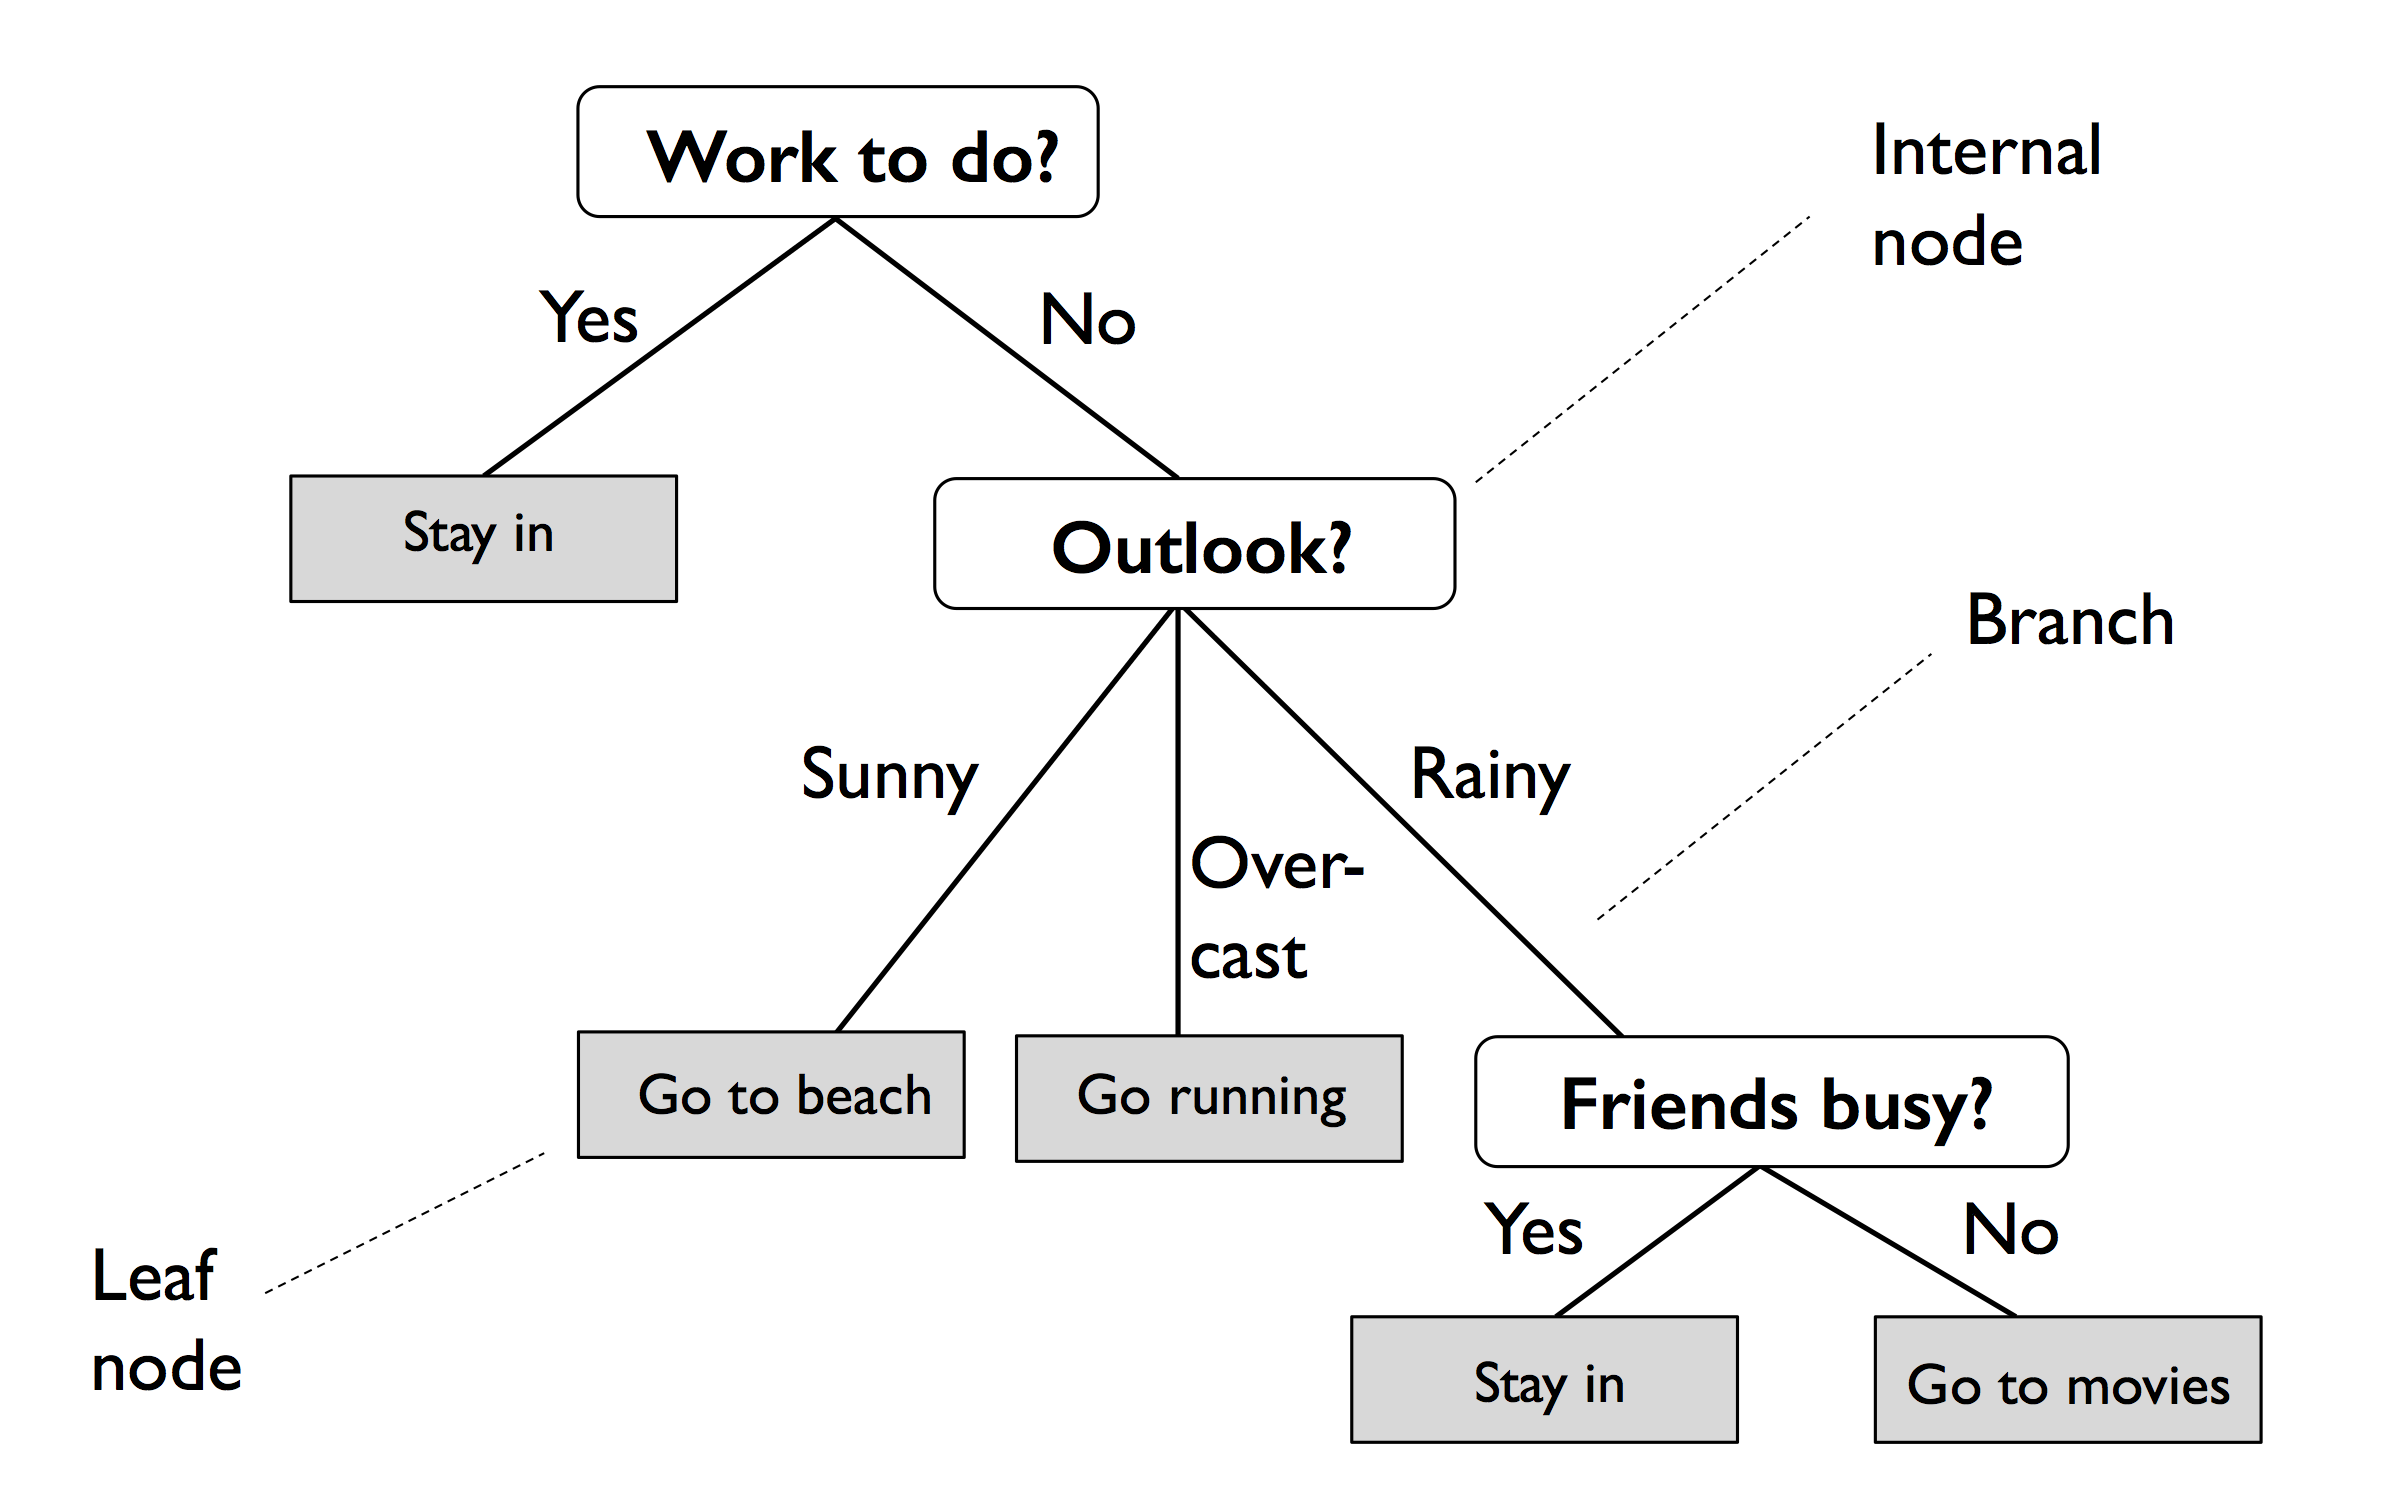
\includegraphics[width=80mm]{img/day03/fig01.png}
        \end{center}
    \end{figure}
\end{frame}

\begin{frame}{決定木}
    決定木アルゴリズムの手順をを示すと以下のようになる。
    \vspace{1em}
    \begin{enumerate}
        \item 木の根(root)から初めて、情報利益(分割された集合の要素についてのばらつきの減少)が最大になる特徴量で分割する。
        \item 末端ノード(reaf)が純粋になるまでreafを分割し続ける。
    \end{enumerate}
    \vspace{1em}
    ここで、reafが単純になるということは各reafの訓練データがすべて同じクラスに属することを示す。 \\
    reafを分割し続けると、木がとても深くなるので深くなりすぎないように、深さに
    制限を設けて木を剪定(prune)する必要がある。
\end{frame}

\begin{frame}{情報利益の最大化}
    最も情報利益の高いノードで分割するには、最適化の対象を定義すべきである。
    この目的関数は分割ごとの利益情報\(IG\)が最大となるように定式化して、以下のように表せる。
    \begin{equation*}
        IG(D_p, f) = I(D_p) - \sum_{j=1}^{m} \frac{N_j}{N_p} I(D_j)
    \end{equation*}
    ここで、\(f\)は分割を行う特徴量であり、\(D_p\)は親のデータセット、\(D_j\)はj番目の
    子ノードのデータセットである。\(I\)は不純度を数値化したものであり、
    \(N_p\)は親ノードのデータの個数、\(N_j\)は子ノードのデータの個数である。\\
    つまり、情報利益とは「親ノードの不順度」と「子ノードの不順度の合計」の差であり、
    子ノードの不純度が低いほど、情報得利益は大きくなる事がわかる。
\end{frame}

\begin{frame}{情報利益の最大化}
    話を単純にするためと、組み合わせ探索空間を減らすために、ほとんどのライブラリでは
    二分決定木を実装している。つまり親ノードは\(D_{left}\)と\(D_{righ}\)の2つの子ノードに分かれる。
    \begin{equation*}
        IG(D_p, f) = I(D_p) - \frac{N_{left}}{N_p}I(D_{left})- \frac{N_{right}}{N_p}I(D_{right})
    \end{equation*}
\end{frame}

\begin{frame}{エントロピー}
    二分決定木でよく使われる不順度の指標または分類条件はジニ不純度(Gini impurity; \(I_G\))、
    エントロピー(entropy; \(I_H\))、分類誤差(classfication error; \(I_E\))の3つである。\\
    ここでは空でないクラス\(i\)(\( p(i \mid t)\neq 0\))のを対象にエントロピーの定義から始める。
    \begin{equation*}
        I_H(t) = - \sum_{i=1}^{c}p(i \mid t)log_2P(i \mid t)
    \end{equation*}
    \(p(i \mid t)\)は、特定のノード\(t\)においてクラスiに属しているデータの点の割合を表している。
    二値分類の場合、データが完全に分離している場合はエントロピーは\(0\)となり、一様に分布している場合は
    エントロピーは\(1\)となる。
    \begin{equation*}
        I_H(t) = 
        \begin{aligned}
            & \left\{ \,
                \begin{aligned}
                    & 1 & \quad &(p(i=0 \mid t) = 1.0, p(i=1 \mid t) = 0.0) \\
                    & 0 & \quad &(p(i=0 \mid t) = 0.5, p(i=1 \mid t) = 0.5)
                \end{aligned}
            \right.
        \end{aligned}
    \end{equation*}
    よって、エントロピーは相互情報量(2つの確率の依存度)を最大化する試みだと言える。
\end{frame}

\begin{frame}{ジニ不純度}
    ジニ不純度については、誤分類の確率を最大化する条件であると解釈できる。
    \begin{equation*}
        I_G(t) = \sum_{i=1}^{c}p(i \mid t)(1-p(i \mid t)) = 1 - \sum_{i=1}^{c}p(i \mid t)^2
    \end{equation*}
    エントロピーと同様に、ジニ不純度が最大になるのは、クラスが完全に混合している場合である。
    例として、二値分類の場合(\(c=2\))の場合は次のようになる。
    \begin{equation*}
        I_G(t) = 
        \begin{aligned}
            & \left\{ \,
                \begin{aligned}
                    & 1 - 1^2 - 0^2 = 0 & \quad &(p(i=0 \mid t) = 1.0, p(i=1 \mid t) = 0.0) \\
                    & 1 - 0.5^2 - 0.5^2 = 0.5 & \quad &(p(i=0 \mid t) = 0.5, p(i=1 \mid t) = 0.5)
                \end{aligned}
            \right.
        \end{aligned}
    \end{equation*}
    一般的にはジニ不純度はエントロピーとよく似た結果をになることが知られている。
\end{frame}

\begin{frame}{分類誤差}
    もう一つの分類誤差は木の剪定には役に立つ条件だが、ノードのクラス確率の変化にはあまり
    敏感ではないので木を成長させるのには適していない。
    \begin{equation*}
        I_E = 1 - \max(p(i \mid t))
    \end{equation*}
    このことを理解するために下図の例を用いて不純度条件を計算していく。
    \begin{figure}[b]
        \begin{center}
        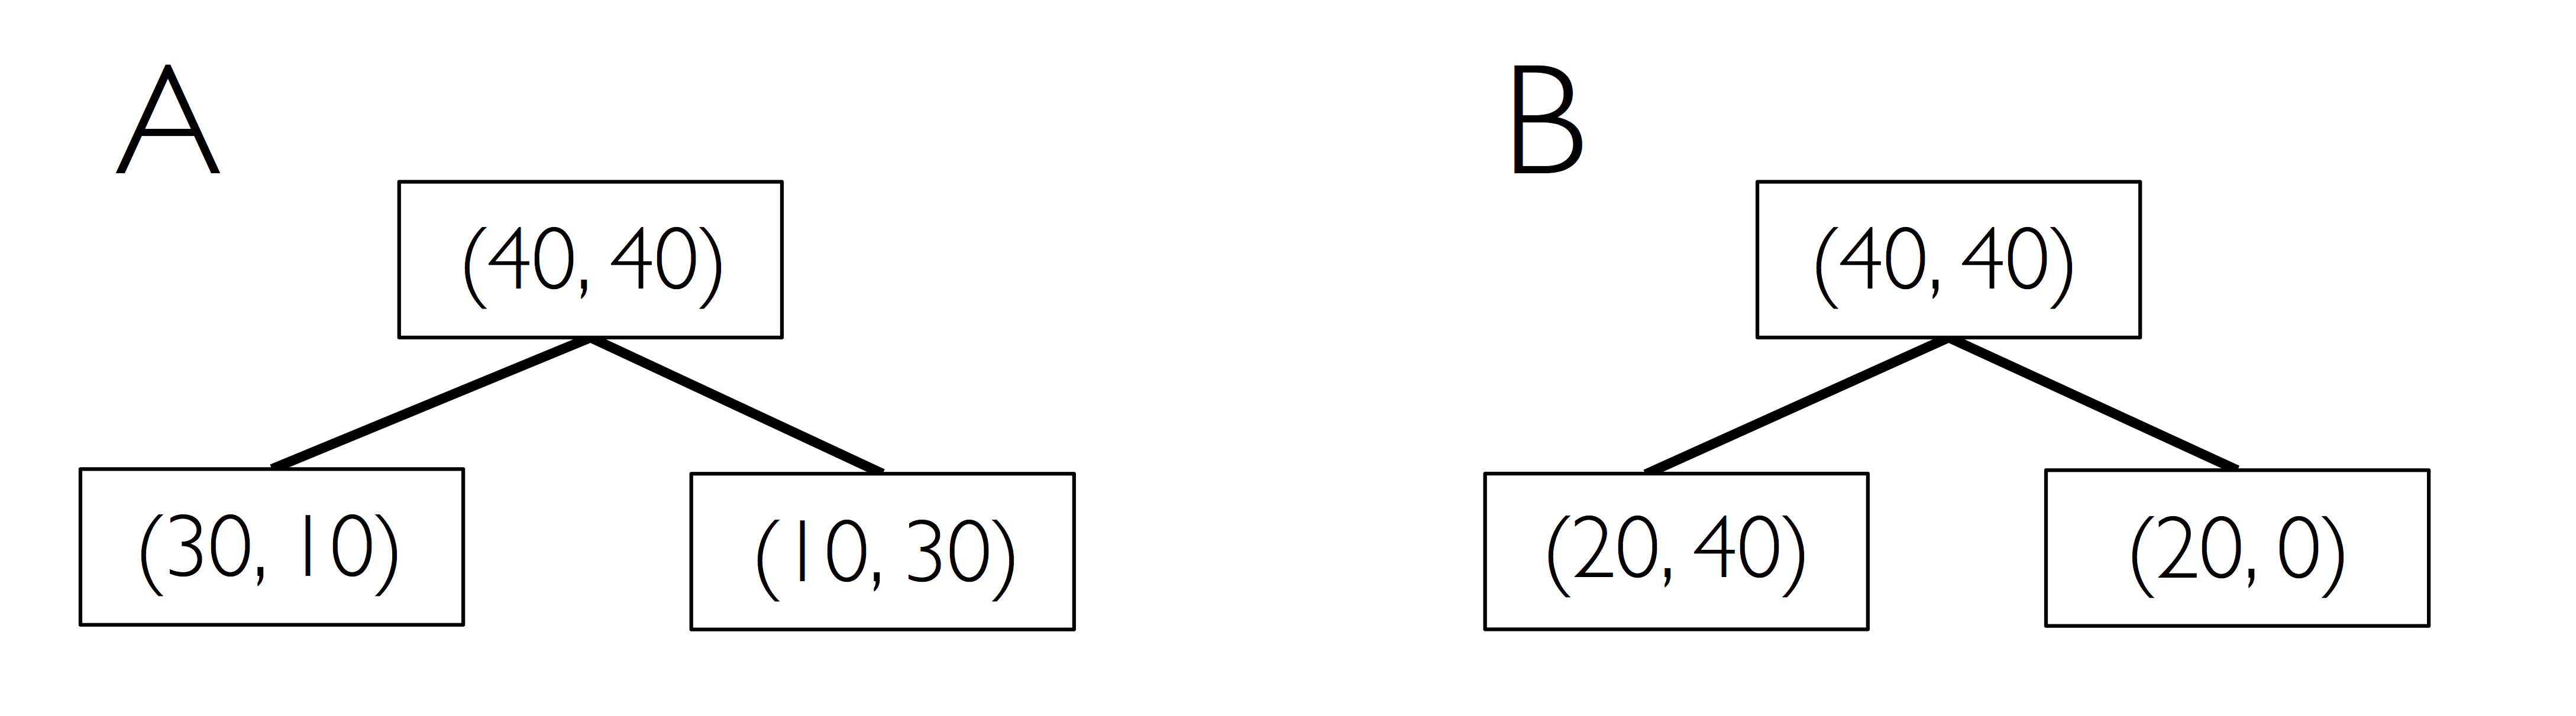
\includegraphics[width=100mm]{img/day03/fig02.png}
        \end{center}
    \end{figure}
\end{frame}

\begin{frame}{不純度関数の可視化}
    最後に各不純度条件をクラス1の確率範囲(\(0\leq p \leq 1\))のグラフにプロットして、視覚的に比較してみる。
    その際に、Entropyのみが最大値が1なので、他の不順度関数と比較できるようEntropyを0.5倍したEntropy(sclaled)を追加した。
    \vspace{1em}
    \begin{figure}[b]
        \begin{center}
        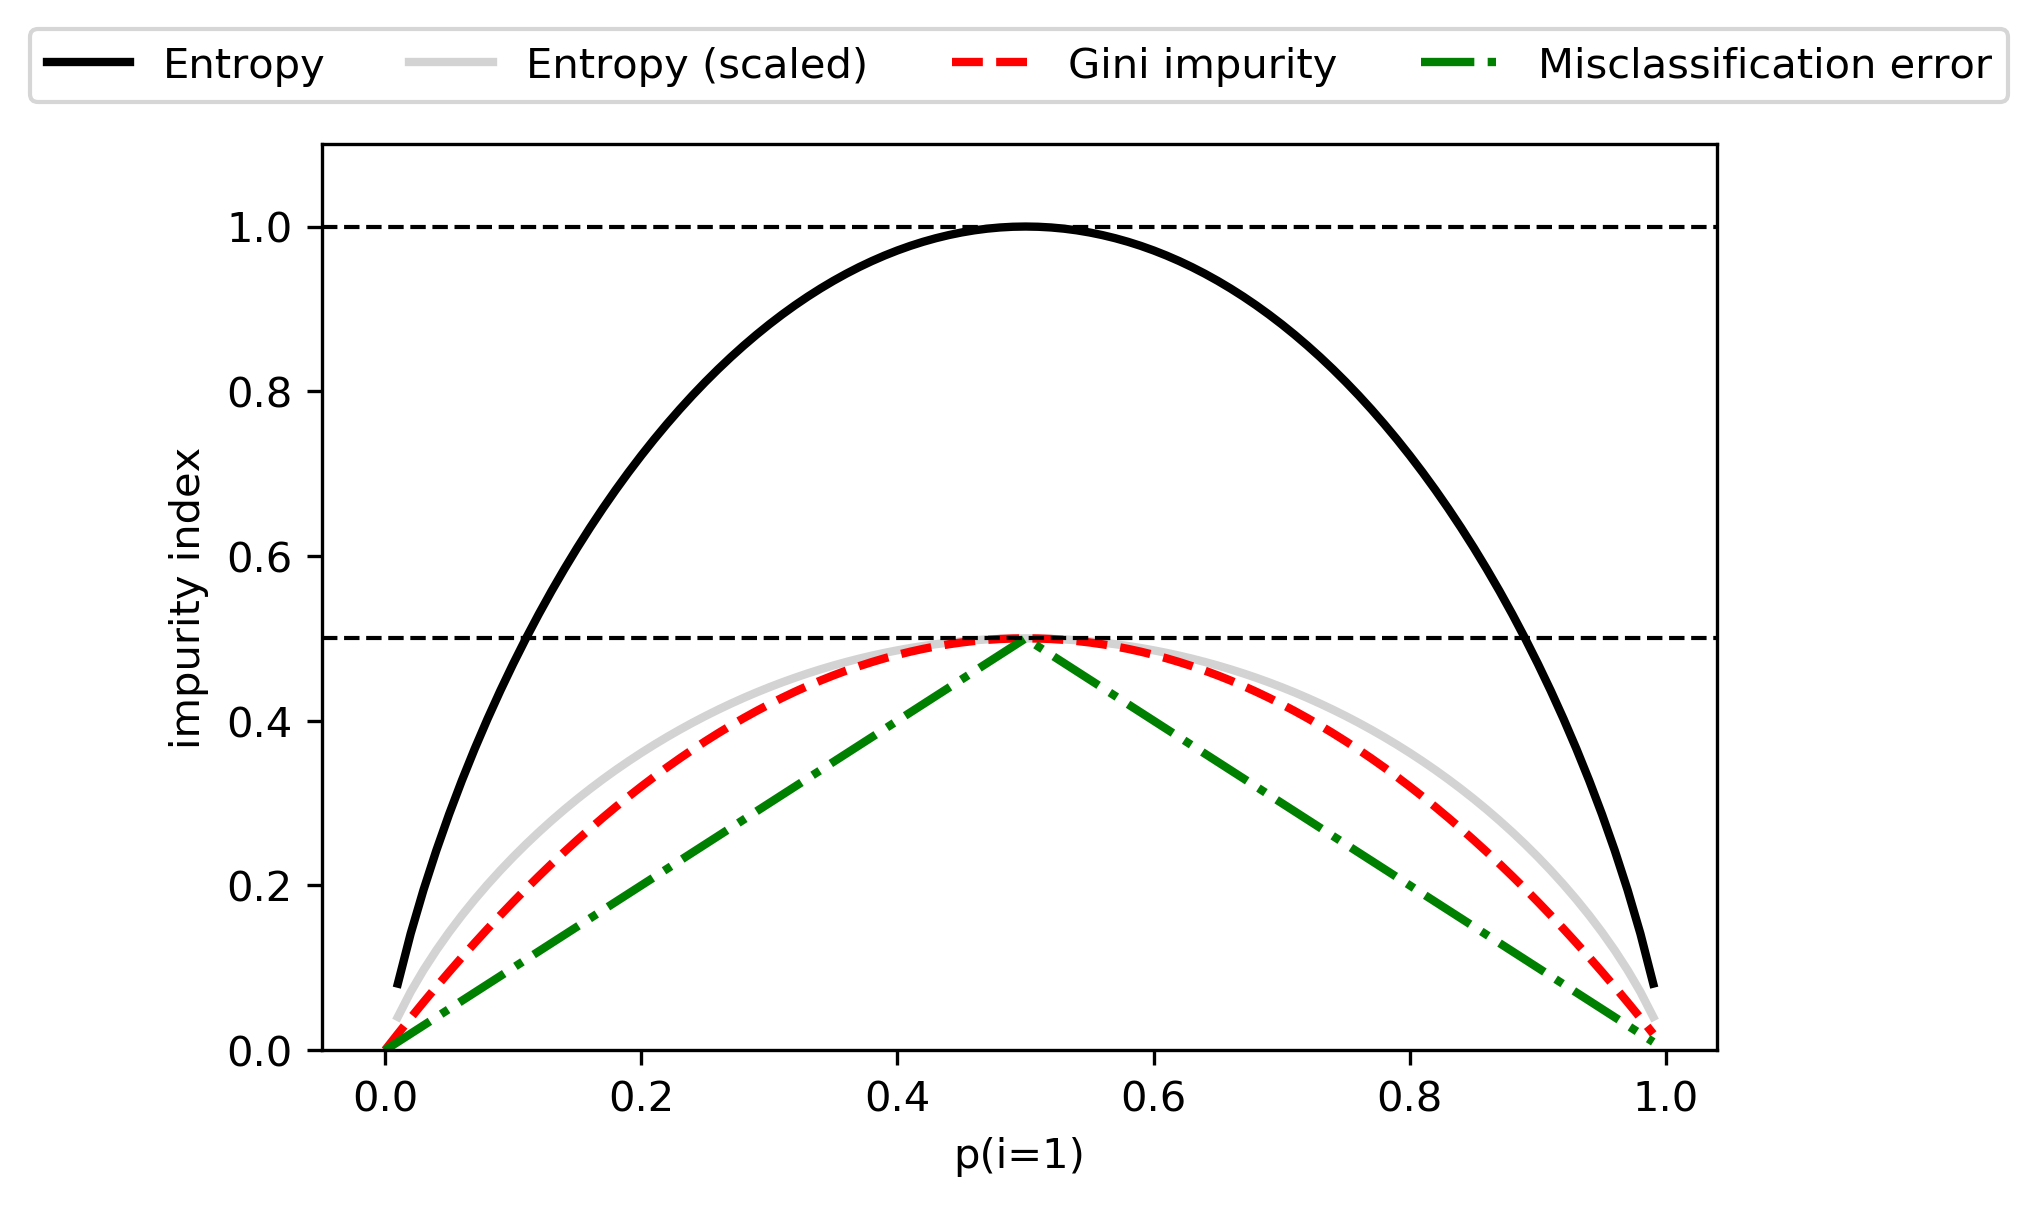
\includegraphics[width=85mm]{img/day03/fig03.png}
        \end{center}
    \end{figure}
\end{frame}

\section{ランダムフォレスト}
\begin{frame}{ランダムフォレスト}
    アンサンブル法は、その分類性能の高さと過学習に対する堅牢性から、絶大な人気を獲得している。
    決定木のアンサンブルであるランダムフォレストはそれぞれバリアンスが高い複数の(深い)決定木を平均化することによって、より汎化性能が高く、
    過学習に強いモデルとなっている。
    \vspace{1em}
    \begin{enumerate}
        \item 訓練データからランダムに\(n\)個のデータ(ブートストラップ標本)を復元抽出する。
        \item ブートストラップ標本から決定木を成長させる。各ノードで以下を行う。
        \begin{enumerate}
            \item d個の特徴量をランダムに非復元抽出する。
            \item 情報利得を最大化することにより、最適な分割となるようにノードを分割する。
        \end{enumerate}
        \item ②の手順①,②を\(k\)回繰り返す。
        \item 決定木ごとの予測をまとめ、多数決によって最終的なクラスラベルを割り当てる。
    \end{enumerate}
    \vspace{1em}
    \rightline{\footnotesize ※復元抽出: 重複を許して選択すること}
\end{frame}

\section{k最近傍方}
\begin{frame}{k最近傍方}
    最後に説明する教師あり学習アルゴリズムはk最近傍(k-nearest neighbor classfire: KNN)である。
    KNNは怠惰学習(lazy learner)の代表的な例である。「怠惰」と呼ばれる理由は訓練データから
    判別関数を学習せずに訓練データセットを暗記するためである。
\end{frame}

\begin{frame}{k最近傍方}
    KNNのアルゴリズムは単純であり、以下の手順にまとめることができる。
    \vspace{1em}
    \begin{enumerate}
        \item \(k\)の値と距離指標を選択する。(ユーグリット距離、マンハッタン距離等)
        \item 分類したいデータ点から\(k\)個の最近傍のデータを点を見つけ出す
        \item 多数決によりクラスタベルを割り当てる。
    \end{enumerate}
    \begin{figure}[b]
        \begin{center}
        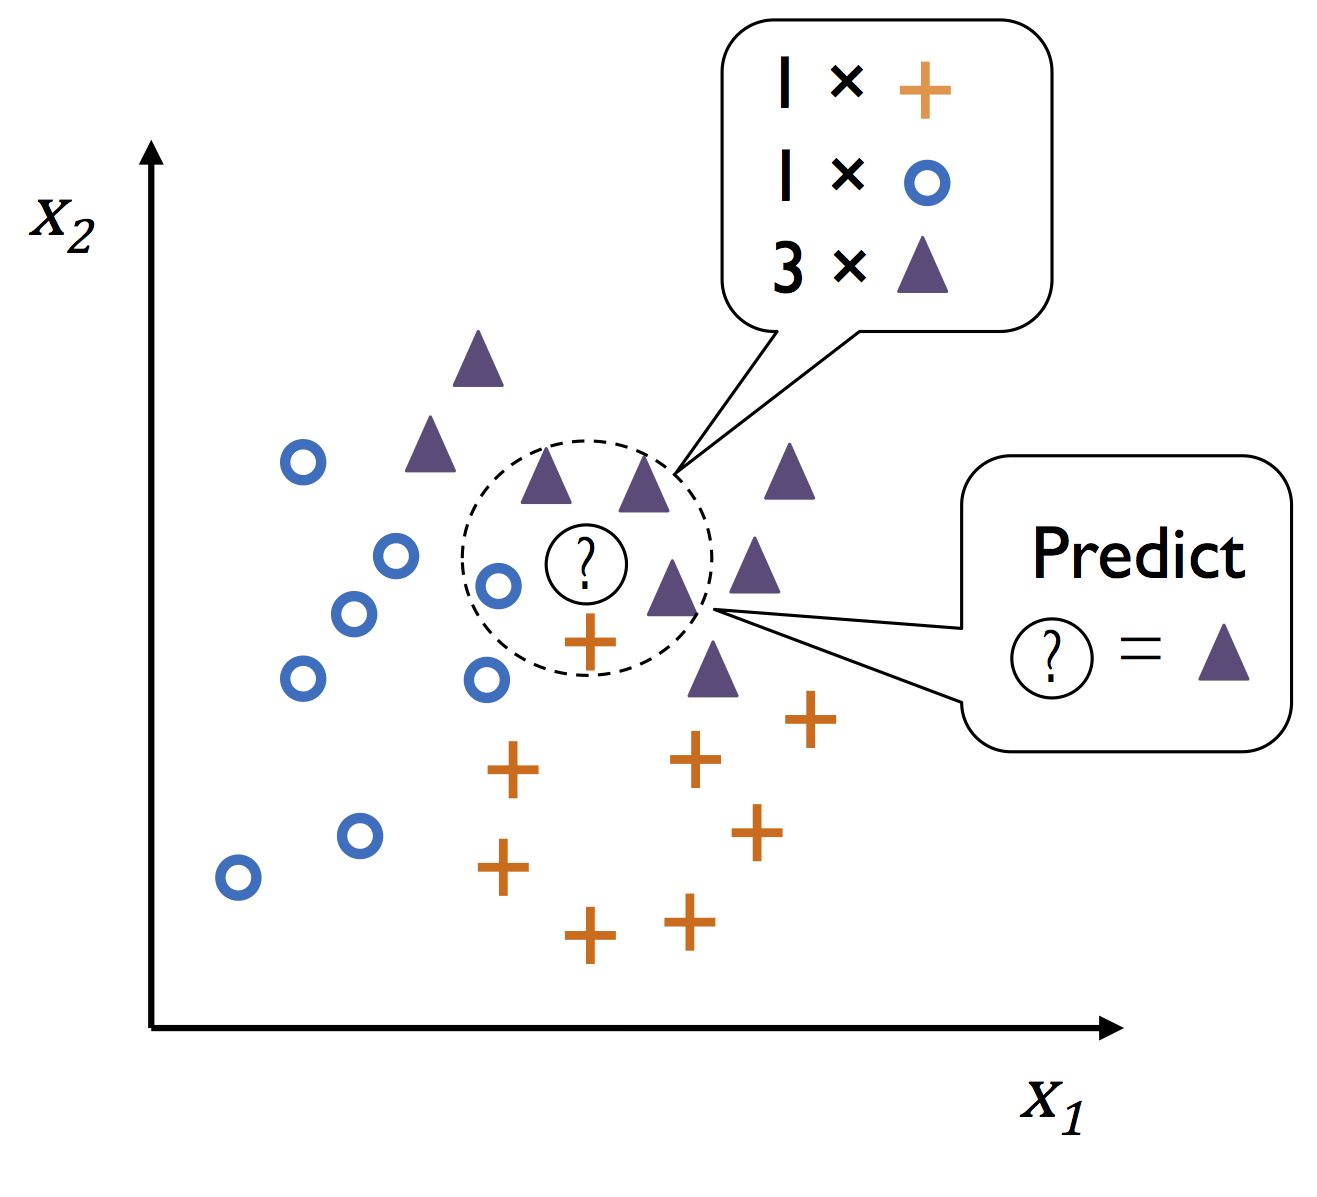
\includegraphics[width=50mm]{img/day03/fig04.png}
        \end{center}
    \end{figure}
\end{frame}

\end{document}